\begin{frame}{GUI to simplify the usage of snakemake}
    \begin{columns}
        \begin{column}{0.5\textwidth}

            \only<1>{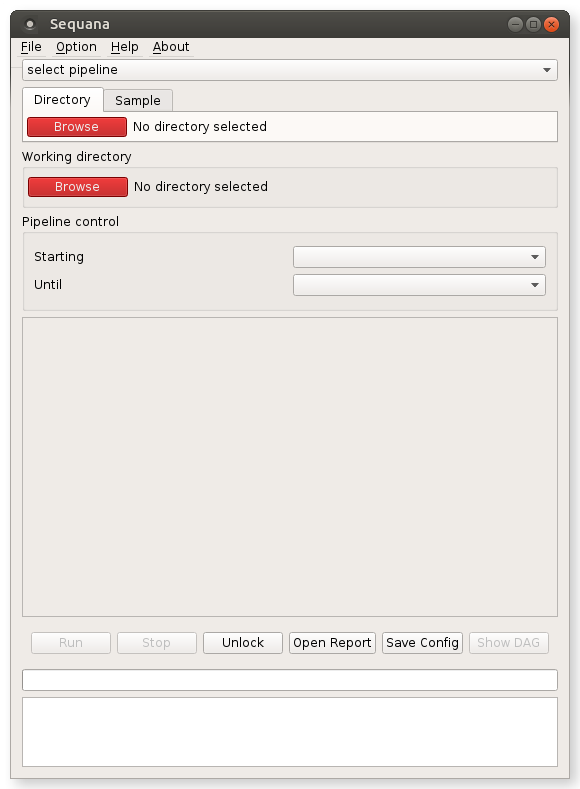
\includegraphics[scale=0.25]{../../images/sequana_init}}

            \only<2>{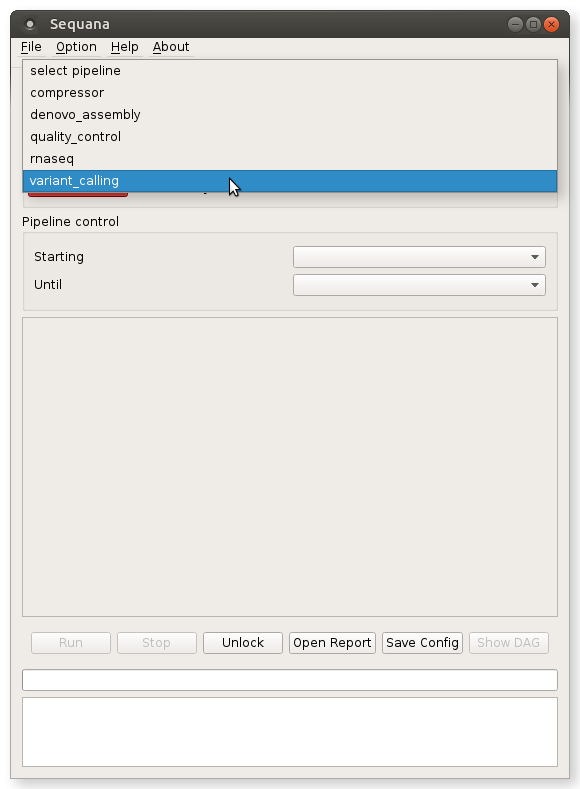
\includegraphics[scale=0.25]{../../images/choose_pipeline}}

            \only<3>{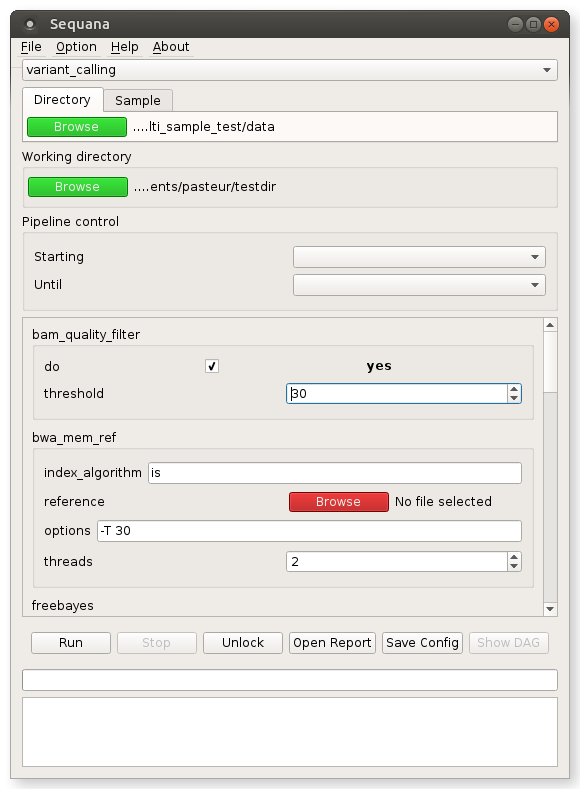
\includegraphics[scale=0.25]{../../images/choose_input_output}}

            \only<4>{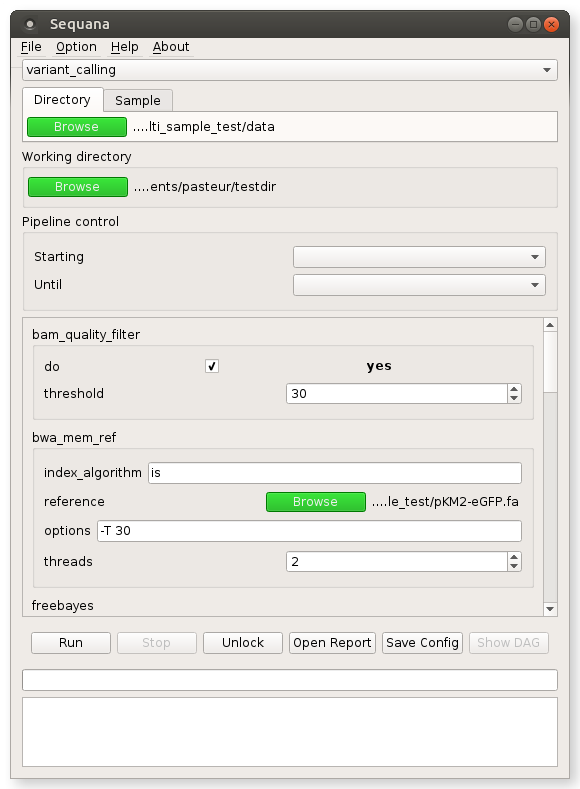
\includegraphics[scale=0.25]{../../images/sequana_pipeline}}

            \only<5>{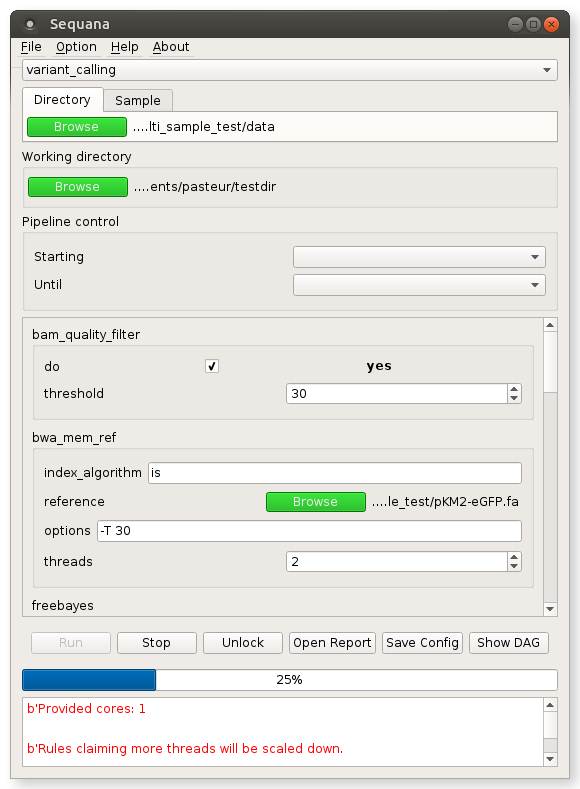
\includegraphics[scale=0.25]{../../images/sequana_running}}

            \only<6>{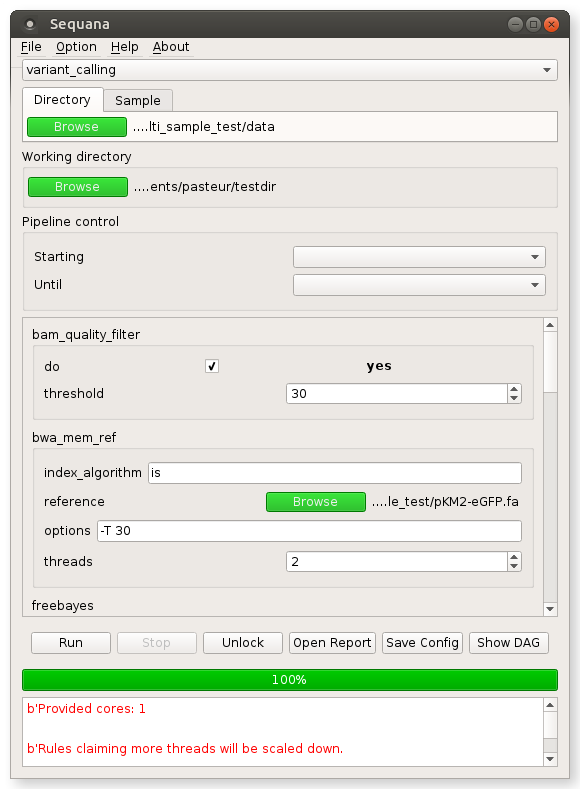
\includegraphics[scale=0.25]{../../images/sequana_finish}}

        \end{column}
        \begin{column}{0.5\textwidth}
            \only<1>{
                \begin{itemize}
                    \item Interface developed with PyQT5 and python
                    \item Wrap our snakemake pipelines to ease the usage
                    \item Usable on our cluster, which allows X11
                \end{itemize}
            }
            \only<2-6>{
            \begin{enumerate}
                \item<2-6> Choose a pipeline
                \item<3-6> Set input and output
                \item<4-6> Fill the config formular
                \item<5-6> Run the pipeline
                \item<6> Finished !
            \end{enumerate}
            }
        \end{column}
    \end{columns}
\end{frame}

